\let\negmedspace\undefined
\let\negthickspace\undefined
\documentclass[journal]{IEEEtran}
\usepackage[a5paper, margin=10mm, onecolumn]{geometry}
\usepackage{lmodern} % Ensure lmodern is loaded for pdflatex
\usepackage{tfrupee} % Include tfrupee package

\setlength{\headheight}{1cm} % Set the height of the header box
\setlength{\headsep}{0mm}     % Set the distance between the header box and the top of the text

\usepackage{gvv-book}
\usepackage{gvv}
\usepackage{cite}
\usepackage{amsmath,amssymb,amsfonts,amsthm}
\usepackage{algorithmic}
\usepackage{graphicx}
\usepackage{textcomp}
\usepackage{xcolor}
\usepackage{txfonts}
\usepackage{listings}
\usepackage{enumitem}
\usepackage{mathtools}
\usepackage{gensymb}
\usepackage{comment}
\usepackage[breaklinks=true]{hyperref}
\usepackage{tkz-euclide} 
\usepackage{listings}
\usepackage{gvv}                                        
\def\inputGnumericTable{}                                 
\usepackage[latin1]{inputenc}                                
\usepackage{color}                                            
\usepackage{array}                                            
\usepackage{longtable}                                       
\usepackage{calc}                                             
\usepackage{multirow}                                         
\usepackage{hhline}                                           
\usepackage{ifthen}                                           
\usepackage{lscape}
\usepackage{circuitikz}
\tikzstyle{block} = [rectangle, draw, fill=blue!20, 
    text width=4em, text centered, rounded corners, minimum height=3em]
\tikzstyle{sum} = [draw, fill=blue!10, circle, minimum size=1cm, node distance=1.5cm]
\tikzstyle{input} = [coordinate]
\tikzstyle{output} = [coordinate]


\begin{document}

\bibliographystyle{IEEEtran}
\vspace{3cm}

\title{2.6.39}
\author{AI25BTECH11028-R.Manohar}
 \maketitle
{\let\newpage\relax\maketitle}

\renewcommand{\thefigure}{\theenumi}
\renewcommand{\thetable}{\theenumi}
\setlength{\intextsep}{10pt} % Space between text and floats


\numberwithin{equation}{enumi}
\numberwithin{figure}{enumi}
\renewcommand{\thetable}{\theenumi}

\textbf{Question}:
The area of the quadrilateral ABCD, where $\vec{A}(0,4,1), \vec{B}(2,3,-1), \vec{C}(4,5,0)$ and $\vec{D}(2,6,2)$, is equal to

\textbf{Solution:}  
The area of a quadrilateral is given by half the magnitude of the cross product of its diagonals.  

First, we find the vectors for the diagonals  
\begin{align*}
 \vec{P} &= \vec{C} - \vec{A} = \myvec{4\\5\\0} - \myvec{0\\4\\1} = \myvec{4\\1\\-1} \\
 \vec{Q} &= \vec{D} - \vec{B} = \myvec{2\\6\\2} - \myvec{2\\3\\-1} = \myvec{0\\3\\3} 
\end{align*}

Now, we compute the cross product $\vec{P} \times \vec{Q}$ using the determinant expansion:  

\begin{align*}
\vec{P} \times \vec{Q} &= 
\myvec{
\left|\myvec{1 & 3 \\ -1 & 3}\right| \\
-\left|\myvec{4 & 3 \\ -1 & 3}\right| \\
\left|\myvec{4 & 1 \\ 0 & 3}\right|
} \\
&= \myvec{(1)(3) - (3)(-1) \\ -( (4)(3) - (3)(-1)) \\ (4)(3) - (1)(0)} \\
&= \myvec{6 \\ -12 \\ 12}
\end{align*}

The area is half the magnitude of this vector:  

\begin{align*}
\text{Area} &= \frac{1}{2} \|\vec{P} \times \vec{Q}\| \\
&= \frac{1}{2} \sqrt{6^2 + (-12)^2 + 12^2} \\
&= \frac{1}{2} \sqrt{36 + 144 + 144} \\
&= \frac{1}{2} \sqrt{324} \\
&= \frac{1}{2}(18) \\
&= 9
\end{align*}

Thus, the area of the quadrilateral is 9 square units.

\centering
    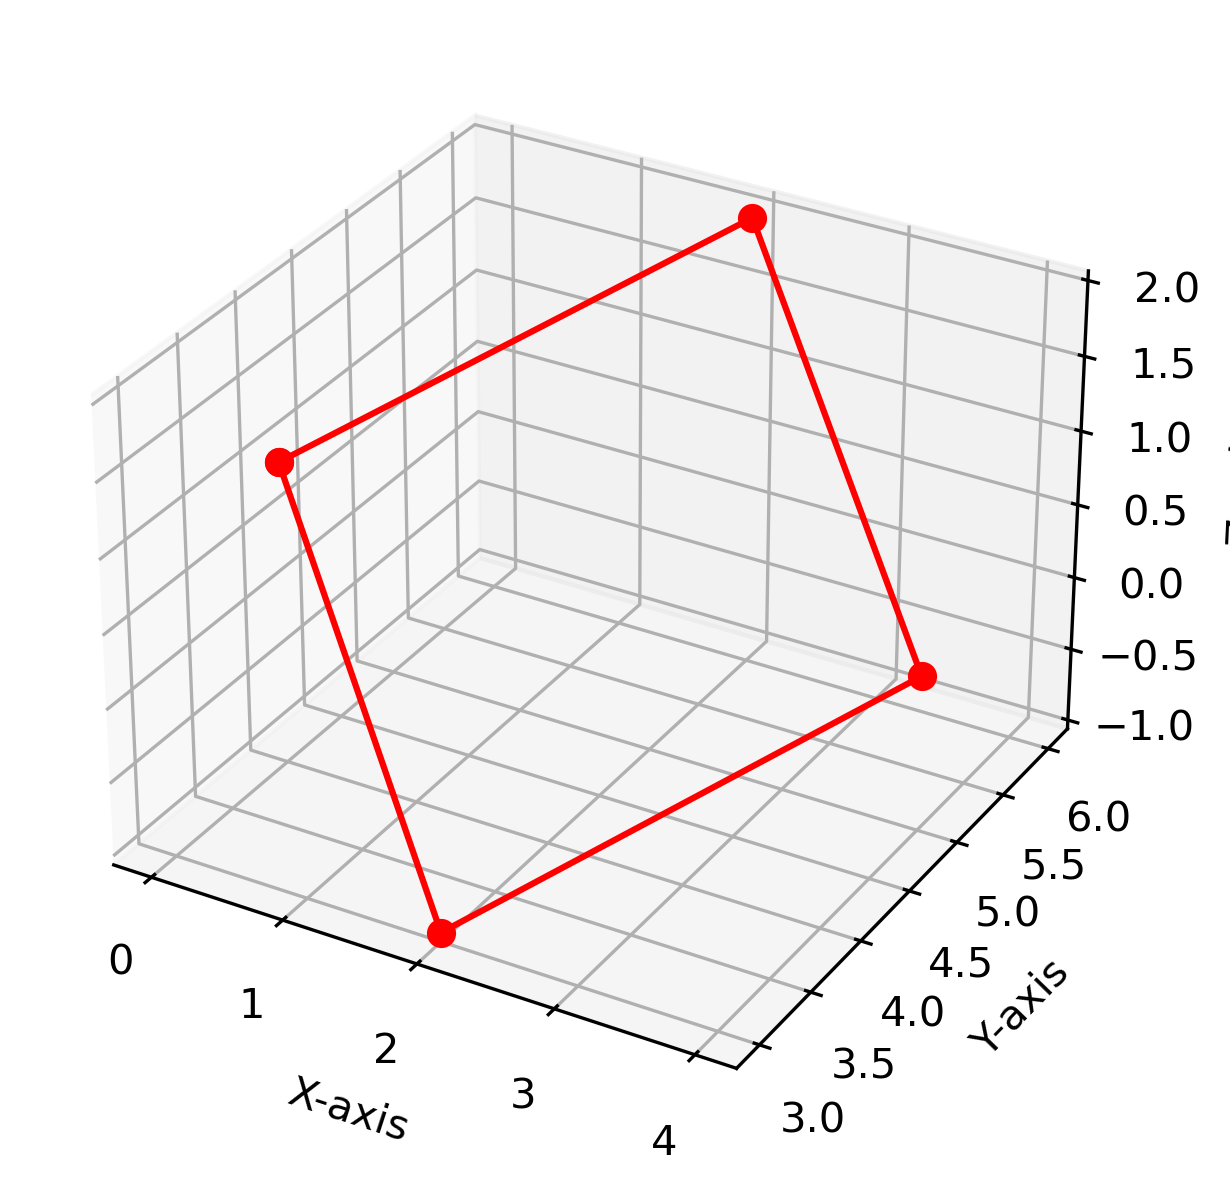
\includegraphics[width=\columnwidth, height=0.8\textheight, keepaspectratio]{figs/Figure_1.png}

\end{document}
